\subsection{Know your user}

Assisting the user - our client - is our primary purpose. \\

We must be aware of the needs of our users in order to meet their demands, as well as being aware of deficiencies in the market, so we can cover any 'holes'.
In the case of public-good data, you also need to consider how to meet the needs of certain groups of users who might be disadvantaged in some way.\\

% TODO: not sure what this means.
% Whether our target audience is unique, that is, take all types of users equally, considering the
% average user, as for a characteristic user, we should know the homogeneous characteristics of our group.\\

So you will need access to information on the psychological, social and economic characteristics of your target users, to ascertain not only
their needs, but also their wishes and preferences.\\

It is important to have a feedback process, both to ensure that your objectives are met, as well as to indicate how you can improve your offering.
This feedback process might be passive i.e. by collecting page and traffic data, or it might be explicit, through the use of explicit feedback requests
and/or surveys.\\

\subsubsection*{Suggested strategies} 

\begin{itemize}
    \item Define the characteristics of your users. Study both their characteristics and the situation of the
    market.
    \item Use a mechanism that helps us obtain feedback, either by a system of points, test or
    an automatic mechanism that allows tracking the behaviour of the user. We can also choose the combination of both
    options.
\end{itemize}

\subsubsection*{In the context of Aire Guru \ldots}

Air Guru is aimed at the general population, therefore it is appropriate to present fully analysed information in the simplest way possible.
In addition, we pay special attention to users who may have a
disease or medical condition, caused or affected by air pollution.\\

We mentioned previous that we discovered a number of deficiencies in existing websites. In addition the following specific gaps in functionality were discovered:

\begin{itemize}
    \item No ability to track exposure over time. We are interested to know the level of pollution we are exposed over the long term, not only at a specific instant.
    \item Overly complicated presentation, suitable more for further analysis than presentation to the general public.
    \item No of explanation of the consequences of pollution exposure, particularly their influence on health or medical conditions.
\end{itemize}

Once Aire Guru was operational, we tested it with 14 identified users. Our website integrates Google Analytics that allow us to evaluate
user behaviour, how many pages they access, and how long they stay on each page.
After testing, we surveyed the users to measure not only the level of overall satisfaction with the website,
but also to verify the utility and determine if the user was able to achieve their objective.\\

Thanks to Aire Guru, users noticed about medical conditions with the potential to affect them personally, that could be caused or made worse by air pollution.\\

\begin{figure}[ht]
    \centering
    \subfigure[Aire Guru Form]
        {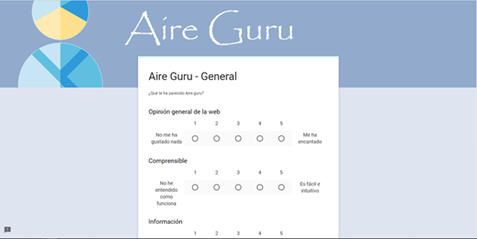
\includegraphics[width=5.5cm  ]{form}}
    \hfill
    \subfigure [Google Analytics]
        {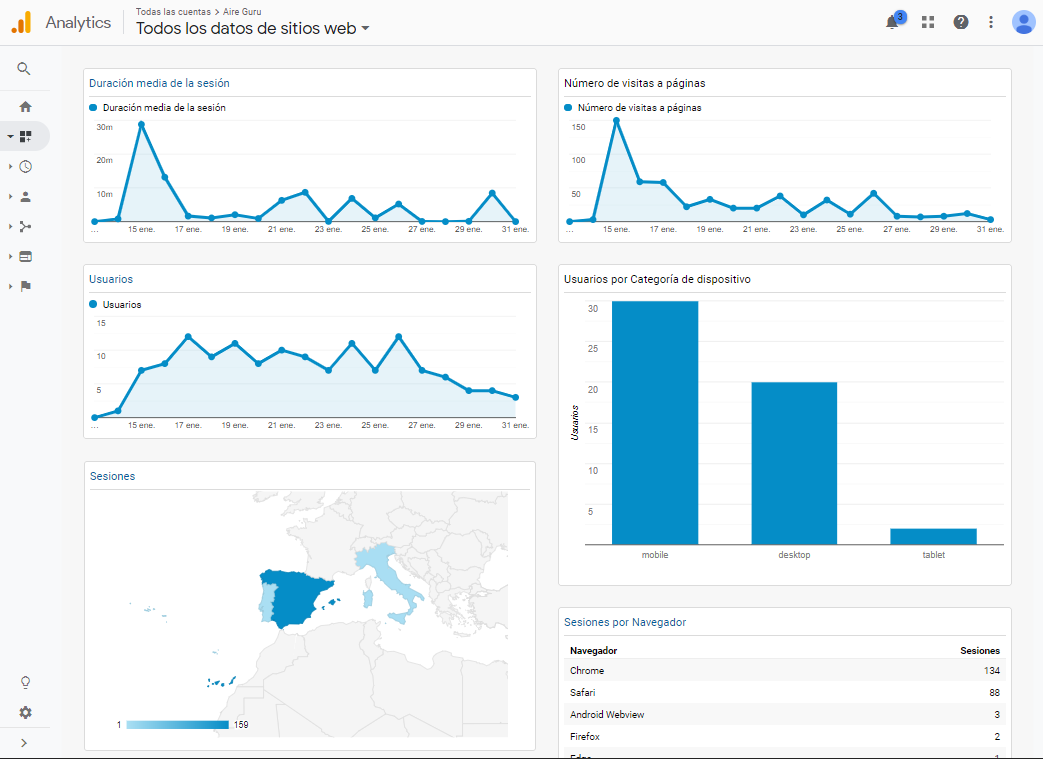
\includegraphics[width=5.5cm]{Figure_3_2_1_userFeedback}}
    \caption{User Feedback}
\end{figure}

\begin{center}
    \bf{Figure 3.2.1. User Feedback}
\end{center}